\documentclass[border=10pt]{standalone}
%%%<
\usepackage{verbatim}
%%%>

\usepackage{tikz}
\usetikzlibrary{arrows.meta}
\tikzset{%
  >={Latex[width=2mm,length=2mm]},
  % Specifications for style of nodes:
            base/.style = {rectangle, rounded corners, draw=black,
                           minimum width=4cm, minimum height=1cm,
                           text centered, font=\sffamily, fill=white},
           dc/.style = {base,dashed}
}
\begin{document}    
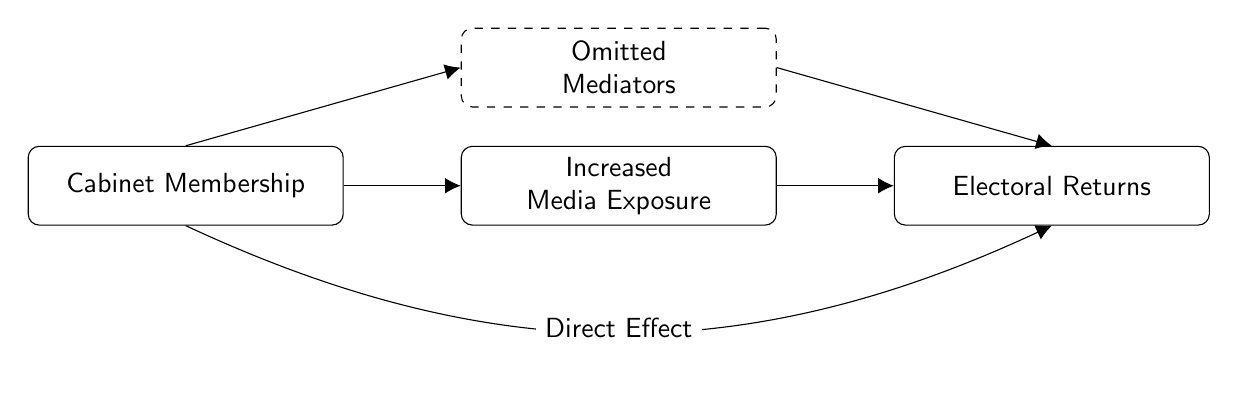
\begin{tikzpicture}[node distance=1.5cm,
    every node/.style={fill=white, font=\sffamily}, align=center]
    

  % Specification of nodes (position, etc.)
  \node (start)		[base]		{Cabinet Membership};
  \node (media)		[base, right of=start, xshift=4cm]		{Increased \\ Media Exposure};
  \node (mediator)	[dc, above of=media]	{Omitted \\ Mediators};
  \node (electoral)	[base, right of=media, xshift=4cm]	{Electoral Returns};
  
  % Specification of lines between nodes specified above
  % with additional nodes for description 	
  \draw[->]             (start) -- (media);
  \draw[->]		    (start.north) -- (mediator.west);
  \draw[->]		    (start.south) to [out=335, in=205] (electoral.south);
  \draw[->]		    (media) -- (electoral);
  \draw[->]		    (mediator.east) -- (electoral.north);
  
  \node (direct)		[below of=media, fill=white, color=white, text=black, yshift=-0.3cm] {Direct Effect};
  \end{tikzpicture}
\end{document}